% !TEX root = main.tex

\section{Symbolic execution of binary code}

The importance of performing symbolic analysis of a program's properties on binary code is on the rise for a number of reasons. Binary code analysis is attractive as it reasons on code that will actually execute: not requiring source code significantly extends the applicability of such techniques (to, e.g., common off-the-shelf proprietary programs, firmwares for embedded systems, malicious software), and it gives the ground truth important for security applications whereas source code analysis may yield misleading results due to compiler errors and optimizations~\cite{BITBLAZE-ICISS08}. Also, the recent advances in runtimes for programs written in dynamic languages brought just-in-time compilation to the masses, taking over on interpreters used when no efficient source-to-binary translation of code was statically possible. 

Analyzing binary code is commonly seen as a challenging task due to its complexity and lack of a high-level semantics\mynote{[D] I'm omitting obfuscation, code packing, and encryption for now}. Modern architectures offer complex instruction sets: modeling each instruction can be difficult, especially in the presence of multiple side effects on processor flags to determine branch conditions. The second major challenge comes from the lack of the higher-level semantics present in source code, especially when no debugging information is available. Types are not explicitly encoded in binary code: even with register types, it is common to store values from one type and read them as another. Similar considerations can be made for array bounds as well. Also, control-flow graph information is not explicitly available, as control flow is performed through jump instructions at both inter- and intra-procedural level. The function abstraction at the binary level does not exist as we intend it at source-code level: functions can be separated in non-contiguous pieces, and code may also call in the middle of a code block generated for a source-level function.

In the remainder of this section we provide an overview of how symbolic executors can address some of the most significant challenges in the analysis of binary code.

\subsection{Lifting to an Intermediate Representation}
\missing

\begin{figure}[h!]
  \centering
  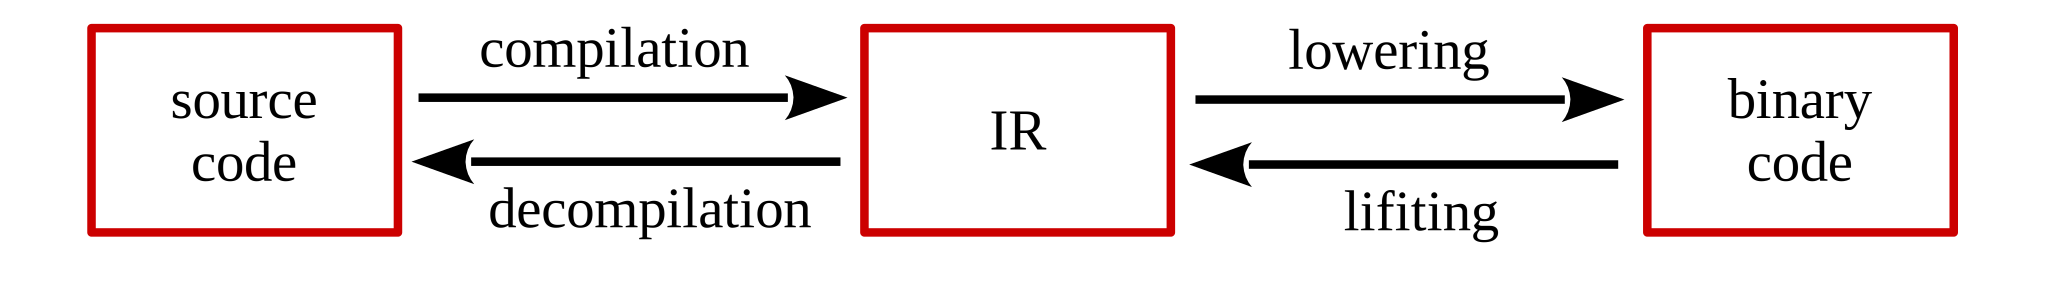
\includegraphics[width=.7\columnwidth]{images/compiler} 
\end{figure}

\vspace{2em}
\mynote{Notes from D\&E start here} For software such as common off-the-shelf programs, neither users nor attackers have access to their source code: 

Challenges (e.g., ~\cite{BITBLAZE-ICISS08}):
\begin{enumerate}
\item Complexity of the instruction sets
\item Lack of a higher-level semantics (functions/CFG, types, buffers)
\item Obfuscation/dynamic code generation
\end{enumerate}

Symbolic techniques may work on the source code or on the binary code. However, it is not uncommon that both the former and the latter work by reasoning on an intermediate representation of the original code. For instance, ~\cite{KLEE-OSDI08} interprets the LLVM bytecode generated by compiling the source code, while~\cite{ANGR-SP16} reasons on the VEX IR that has been obtained by lifting the binary code.

